\chapter{OPTVM}

O OptVM é um sistema que tem o propósito de dar suporte para a migração de VMs em um ambientes de núvens federadas,
isso é feito através \textit{webservices} utilizando o modelo cliente-servidor, mais específicamente o padrão arquitetural 
Representational State Transfer(REST).

O sistema possui dois principais componentes para atingir seu objetivo: um deles, faz uma filtragem de hosts aplicando restrições,
as quais são escolhidas pelo usuário do \textit{webservice}, e o 
outro componente define o melhor subconjunto de hosts de destino para migrar uma VM específica 
baseando-se em objetivos também escolhidos pelo cliente. 
Para a escolha dessas \textbf{restriçoes} e \textbf{objetivos de otimização}, foi dado um nome,
chamado de \textbf{política}. 

As \textbf{restrições}, nada mais são do que regras de negócio que o usuário da API consegue definir através de uma política.
As restrições no OptVM são pré-definidas, ou seja, não são dinâmicas, e elas devem ser apenas escolhidas pelo 
usuário da API. Essa escolha das restrições é feita através das políticas.

Os \textbf{objetivos da otimização}, são interesses do usuário, por exemplo, minimização do consumo de energia. Os objetivos,
assim como as restrições, são pré-definidos pelo OptVM e o usuário tem a opção de utilizá-los ou não através das políticas.
No OptVM, os objetivos são representados com funções objetivo (FO), do problema de otimização. Ou seja, internamente são tratados
como funções matemáticas que representam o objetivo para a otimização.

Por lidar com conhecimentos específicos, como algoritmos de otimização, consumo de energia, entre outras coisas. 
O OptVM busca ser uma solução caixa preta, onde, o usuário não necessita saber nada sobre o funcionamento interno, 
algoritmos utilizados, etc. Basta utilizar as \textit{Application Programming Interfaces} (APIs) para fazer uso de suas funcionalidades.
A intenção é que o usuário não precise entender sobre como as coisas são feitas internamente para obter as vantagens do uso do OptVM.

Neste capítulo, serão apresentados aspectos gerais em relação a implementação e uso do OptVM. 
No primeiro momento serão mostrados os componentes que integram o sistema. 
Depois disso, técnicas e ferramentas utilizadas, e no final a ideia do funcionamento do serviço e como ele é
implementado.

\section{COMPONENTES}
O OptVM é dividido em dois principais componentes: O aplicador de constraints (\textit{constraint applyier})
e o otimizador(\textit{optmizer}). Os dois componentes estão relacionados, porém são representados e 
aplicados separadamente. 

\section{APLICADOR DE CONSTRAINTS (CONSTRAINT APPLYIER)}

Como citado na introdução do capítulo, o OptVM utiliza restrições pré-definidddas.
Para o entendimento de como funciona as o aplicador de restrições, é importante conhecer os tipos de 
restrições e como elas funcionam.

\subsection{Tipos de restrições (constraints)}

As restrições pré definidas, tem um \textit{alias} para que o usuário do serviço faça a identificação no uso delas.
Os tipos de restrições disponibilizadas pelo OptVM operam em 3 níveis, são eles: \textbf{cloud}, \textbf{datacenter} (DC)
e \textbf{hosts}.

Cada restrição tem uma responsabilidade específica, uma regra de negócio que não deve ser infringida. 
As restrições disponibilizadas e seus respectivos níveis são as seguintes:

\begin{enumerate}
  \item Cloud:
  \begin{enumerate}
    \item @TODO
  \end{enumerate}

  \item DC:
  \begin{enumerate}
    \item \textit{Conflito}: Pode conflitar uma localização, por exemplo, uma VM dos USA, não pode habitar em um host de ISRAEL;
    \item \textit{Custo}: Os custos que irão gerar ultrapassam os parâmetros.
  \end{enumerate}

 \item Host
  \begin{enumerate}
    \item \textit{Dependência}: Depende que o host tenha um sistema operacional(OS) ou hypervisor específico (baseado em seus parâmetros);
    \item \textit{Coabitação}: Dependendo dos parâmetros da constraints, exige que o host seja vizinho (1 hop de distância).
  \end{enumerate}
  
\end{enumerate}

\subsection{Algoritmo}
O \textit{constraint applyier} tem a responsabilidade de remover os hosts que não atendem à
uma ou mais restrições estabelecidas pelo usuário. Como as restrições operam nos 3 níveis,
é importante que algoritmo tenha acesso a um contexto onde obtenha informações sobre as núvens, 
datacenters e hosts disponíveis.

O algoritmo que aplica as constraints, consiste em iterar sobre as constraints ordenadas da mais significativa 
(operam em nível de cloud), para a menos significativa (operam em nível de host), e remover os itens que não atendem as
restrições, após cada iteração.

O pseudocódigo do algoritmo é representado da seguinte maneira:

\clearpage

\begin{algorithm}
    \caption{Constraint Applyier}
    \KwIn{as $constraints$ restrições, $context(Clouds, DCs, Hosts)$ contexto com todas as opções disponíveis}
    \KwOut{$context'(Clouds, DCs, Hosts)$ somente com Clouds/DCs/Hosts que atendem as restrições} 

    $context'\leftarrow context$\\
    \For {$constraints \in constraints$} {
        \If {$c$ é do tipo CLOUD} {
            aplica a $constraints$ nas núvens do contexto\\
            $context'\leftarrow nuvensAtualizadas$\\
        }
        \ElseIf {$constraints$ é do tipo DC} {
            aplica a $constraints$ nas DCs do contexto\\
            $context'\leftarrow datacentersAtualizados$\\
        }
        \ElseIf {$constraints$ é do tipo HOST} {
            aplica a $constraints$ nas Hosts do contexto\\
            $context'\leftarrow hostsAtualizados$\\
        }
    }

\end{algorithm}



A intenção de aplicar as restrições ordenadas das mais significativas
para as menos significativas, é para que diminua o número de iterações.
Pois quando, por exemplo, um datacenter não atende uma restrição, os hosts daquele datacenter 
também não são elegíveis como um possível destino, então, as restrições em nível de host para
os hosts desse determinado datacenter nem devem ser executadas. 

Uma representação visual, de como o algoritmo funcionaria, pode ser vista na Figura \ref{fig:constraintapplyier}. 
A ideia é que funcione semelhante a uma estrutura de árvore, e que quando um nó pai não atende a restrição, 
toda a sub-arvore também não atende. E a avaliação é feita top-down.

\begin{figure}[!htb]
  \centering
  \caption{Exemplo de aplicação das constraints}
  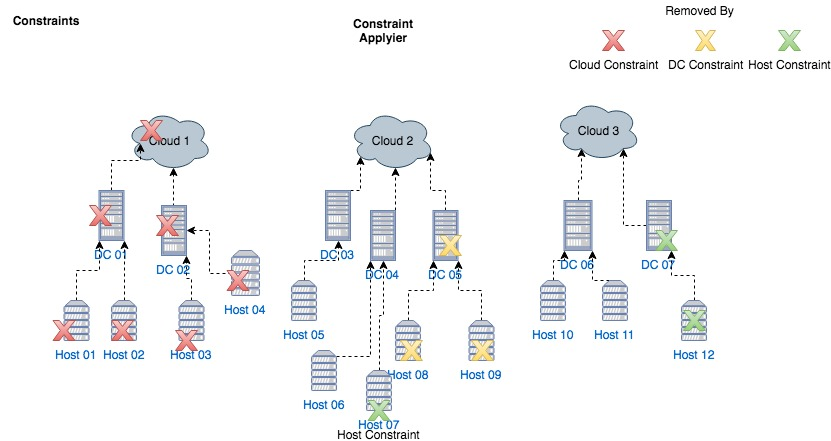
\includegraphics[width=1\textwidth]{./dados/figuras/constraintapplyier}
  \label{fig:constraintapplyier}
\end{figure}

A imagem mostra como as constraints aplicadas em seus respectivos níveis, eliminariam a possíbilidade
da VM migrar para determinado host. Na Figura \ref{fig:constraintapplyier}, foram representados os seguintes casos:

\begin{enumerate}
\item A \textbf{Cloud 1} não atende à alguma restrição escolhida em nível de núvem, então nenhum de seus DCs e por consequência hosts dos DCs, serão alvos válidos;
\item O \textbf{Datacenter 05} não atende alguma restrição em nível de DC, então nenhum de seus hosts estarão disponíveis como alvo de migração;
\item E os \textbf{Host 07 e Host 12} não atendem alguma restrição em nível de host;
\item Um caso mais específico é quando o \textbf{Host 12} não atende a alguma restrição, logo o \textbf{DC 07} não terá nenhum host válido, então também deve ser desconsiderado.
\end{enumerate}

\clearpage

\section{OTIMIZADOR (OPTIMIZER)}

O \textit{optimizer} é responsável por otimizar a seleção dos hosts disponíveis nas núvens da federação
para a VM que necessita migrar. O objetivo é alcançar um melhor subconjunto para a alocação da VM. 
Além disso, a seleção desse subconjunto é selecionado atendendo os objetivos da \textbf{política} 
selecionada para a otimização (conjunto de objetivos e restrições), escolhida pelo usuário.

A otimização feita no OptVM, faz uso de algoritmos genéticos. Os algoritmos genéticos,
são baseados na evolução humana e fazem uso de uma simulação do processo evolutivo descoberto por Darwin.
São feitas diversas avaliações sobre uma população que é iniciada randômicamente no algoritmo. O processo
evolutivo faz com que apenas as soluções com os genes mais aptos "sobrevivam". A aptidão da solução
é dada pela \textit{fitness function}, também chamada de função objetivo.

No OptVM, os objetivos são dinâmicos, ou seja, é possível que o usuário da API escolha por alguns
objetivos e não por outros. Os objetivos disponíveis no OptVM são 3, dos quais um ou mais podem ser 
escolhidos, são eles:

\begin{enumerate}
\item Minimização do consumo de energia;
\item Minimização do tempo de instalação;
\item Minimização da sobrecarga da migração.
\end{enumerate}

Como a otimização possui um conjunto de indivíduos, que formam uma população, cada indivíduo
da população representa uma possível solução para o problema.  Nos algoritmos de 
otimização o indivíduo possui uma representação (\textit{encoding}), que pode ser feita
de diversas maneiras, de maneira binária, por inteiros, entre outros tipos de representação.

Como uma representação representa uma solução para o problema, no OptVM, a 
representação escolhida foi: um array de booleanos que representa cada host.
O valor (\textit{true} ou \textit{false}), se o host está no subconjunto de soluções 
ou não estaria alocada.

\[
  Solution=
  \left[{\begin{array}{cccccc}
    0 & 1 & 0 & 0 & 1 & 0 \\
  \end{array}}\right
  ]
\]

No exemplo, o tamanho escolhido para o subconjunto é de 2 hosts, ou seja, 
a otimização busca achar o melhor subconjunto de 2 hosts. Nesta representação,
os 2 hosts escolhidos na solução, são os hosts 1 e 5 do conjunto de hosts.

\section{COMUNICAÇÃO}
Em termos gerais, uma API é uma interface de software que pode ser chamada e executada \cite{eizinger}. 

Como o OptVM é um serviço que deve ser disponibilizado para uma arquitetura de 
cliente-servidor de maneira distribuída, haviam três possíveis maneiras de implementá-lo, 
que eram REST, SOAP e via chamadas RPC. 
Para o desenvolvimento do OptVM o foi escolhido implementação utilizando o modelo REST. 
A escolha desta opção se deu principalmente pelos seguintes motivos:

\begin{enumerate}
\item É um padrão arquitetural bastante maduro;
\item É agnóstico em relação a liguangens de programação;
\item É bastante flexivel em relação ao modelo de comunicação.
\end{enumerate}

Como o padrão arquitetural REST é agnostico em relação ao formato utilizado para fazer a comunicação dos dados. O \textit{econding} 
dos dados pode ser feito da maneira que for mais conveniente para o usuário. No caso do OptVM é possível fazer a comunicação
tanto no formato XML como no formato JSON.

Isso é controlado pelo próprio cliente da aplicação. É controlado através do cabeçalho \textit{Accept}
da requisição HTTP.

A criação de um recurso de otimização deve-se ser utilizado o seguinte formato, para o corpo da requisição. No exemplo, está sendo
utilizado o formato JSON, porém, o mesmo se aplica também para o XML:

\section{REPRESENTAÇÃO DO SERVIÇO}

O padrão REST, definido por Fielding \cite{fielding}, sugere que se deve criar uma interface para interação com o sistema. 
Essa interface é representada através de recursos, e a interação com esses recursos é feita através de requisições HTTP, 
as quais contém verbos, o corpo da mensagem, cabeçalhos, entre outras informações. Além disso, o padrão arquitetural também sugere que 
haja links para verificar outras informações e tomar ações sobre os recursos, chamado HATEOAS.

\subsection{Recursos}

O OptVM trabalha em cima de 2 recursos, chamados políticas(\textit{policies}) e otimizações(\textit{optimizations}). 
Ambos os recursos, conseguem trabalhar de maneira independente.

O recurso de políticas é responsável por gerenciar (criar, atualizar, deletar), as políticas
cadastradas. As políticas são compostas por objetivos e restrições. 

Já o recurso das otimizações, é responsável por gerenciar as otimizações executadas pelo sistema. O recurso 
além de fazer a otimização, também guarda um histórico, com informações mais detalhadas, 
que pode ser consultado após feitas as otimizações. Além do histórico, o recurso também guarda métricas e informações sobre
a otimização em si, como tempo de execução por exemplo.

Conforme REST propõe, foram utilizados os verbos para realizar as operações correspondentes
ao que eles se propõe a fazer. Então o verbo POST é utilizado para a criação de recursos,
e o GET para a busca de recurso(s), DELETE para deleção e PUT para atualização.

No geral, os recursos do OptVM ficaram organizados da seguinte maneira:

\begin{table}[!htb]
    \centering
    \caption[Recurso Otimização]{Tabela recurso otimização
    \label{tab:tabela-optimization}}
    \begin{tabular}{rrrrr}
        \toprule
            Verbo & URI & Operação \\ 
        \midrule
            GET & \textit{/optimizations} & Todas as otimizações \\
            POST & \textit{/optimizations} &  Cria uma otimização \\
            GET & \textit{/optimizations/:id} & Otimização específica \\
            GET & \textit{/optimizations/:id/details} & Detalhes da otimização \\
            GET & \textit{/optimizations/:id/metrics} & Métricas da otimização \\
        \bottomrule
    \end{tabular}
\end{table}


\begin{table}[!htb]
    \centering
    \caption[Recurso Política]{Tabela recurso policy
    \label{tab:tabela-optimization}}
    \begin{tabular}{rrrrr}
        \toprule
            Verbo & URI & Operação \\ 
        \midrule
            GET & \textit{/policies} & Todas as políticas \\
            POST & \textit{/policies} &  Cria uma política \\
            PUT & \textit{/policies} &  Atualiza uma política \\
            GET & \textit{/policies/:id} & Política específica \\
            DELETE & \textit{/policies/:id} & Exclui específica \\
        \bottomrule
    \end{tabular}
\end{table}



\section{FUNCIONAMENTO DO SERVIÇO}

A utilização do serviço, exige que seja seguido um fluxo. O próprio serviço 
ajuda o usuário seguir o fluxo, através do HATEOAS, indicando links e próximas
ações e consultas que podem ser feitas pelo consumidor da aplicação.

A ideia é que no caso de uso mais simples de utilização do serviço, 
para fazer uma otimização, é seguido o seguinte fluxo:

\begin{enumerate}
 \item Criação de uma política, com seus objetivos e restrições de negócios;
 \item Envio do conjunto de núvens/DCs/Hosts para ser feita a otimização;
 \item Obtenção dos detalhes da otimização.
\end{enumerate}

Apesar do caso de uso básico, é possível utilizar a API de maneiras diferentes,
e fazer as combinações que forem mais úteis para o usuário.

A criação de uma política, é feita enviando os objetivos e as restrições.
Após criada a política, a mesma pode ser utilizada em uma otimização. 

\begin{figure}
  \centering
  \begin{tikzpicture}[
   mybox/.style={
     text width=3cm,
     minimum height=3cm,
     minimum width=3cm,
     node distance=6cm,
     align=center,
     ultra thick,
     draw},
   myarrow/.style={
     ->,
     >=stealth,
     thick
    }
  ]
  \node [mybox](sc) {OptVM};
  \node [mybox,left=of sc] (sp) {Consumidor};
  \draw [myarrow] (sp.east) +(0,1em) coordinate (b1) -- node[above] {criar política} (sc.west |- b1);
  \draw [myarrow] (sp.east) +(0,-1em) coordinate (b1) -- node [above] {criar otimização} (sc.west |- b1) ;
  \draw [myarrow] (sc.west) +(0,-3em) coordinate (b1) -- node [above] {hosts recomendados} (sp.east |- b1) ;
\end{tikzpicture}
\end{figure} 

Após a criação de um política, é possível usá-la para fazer otimizações.

A criação de uma otimização, retorna um objeto com um resumo dos melhores hosts
e sua identificação, para melhorar o destino da VM.
Além disso, é possível obter detalhes de execução, através de \textit{/metrics}, assim
como detalhes da otimização através da URI \textit{/details}.

Um exemplo de \textit{payload} que a criação de uma optimização teria é o seguinte:

\begin{lstlisting}[language=json,firstnumber=1]
{
  "id": 1,
  "policy": 2,
  "clouds": [
    {
      "id": 1,
      "name": "Test",
      "datacenters": [
        {
          "id": 1,
          "hosts": [
            {
              "id": 1,
              "memory": 2000,
              "bandwidth": 1000,
              "vms": [
                {
                  "id": 10,
                  "space": 20,
                  "memory": 150
                }
              ]
            }
          ]
        }
      ]
    }
  ]
}
\end{lstlisting}

E a resposta poderia ter o seguinte formato:

\begin{lstlisting}[language=json,firstnumber=1]
{
  "id": 1,
  "hosts": [
    {
      "cloud": 1,
      "datacenter": 2,
      "host": 1
    }, 
    {
      "cloud": 1,
      "datacenter": 2,
      "host": 1
    }, 
    {
      "cloud": 2,
      "datacenter": 2,
      "host": 4
    }
  ],
  "details": "/optimizations/1/details",
  "metrics": "/optimizations/1/metrics"
}
\end{lstlisting}